\documentclass[]{jsarticle}
\usepackage[dvipdfmx]{graphicx}
\usepackage{fancyvrb}
\usepackage{bm}
\usepackage{listings,jvlisting} %日本語のコメントアウトをする場合jvlisting(もしくはjlisting)が必要
%ここからソースコードの表示に関する設定
\lstset{
  basicstyle={\ttfamily},
  identifierstyle={\small},
  commentstyle={\smallitshape},
  keywordstyle={\small\bfseries},
  ndkeywordstyle={\small},
  stringstyle={\small\ttfamily},
  frame={tb},
  breaklines=true,
  columns=[l]{fullflexible},
  numbers=left,
  xrightmargin=0zw,
  xleftmargin=3zw,
  numberstyle={\scriptsize},
  stepnumber=1,
  numbersep=1zw,
  lineskip=-0.5ex
}

\begin{document}
\section{課題1}
\subsection{課題1-1}
\subsubsection{MAKEユーティリティ}
ウェブサイト\cite{1}によれば,MAKEは,大規模プログラムのコンパイルの簡略化を行うツールである。プログラムが大規模になると,ファイル間の親子関係が複雑になってしまい,コンパイル作業が煩雑になる。そこで,MAKEFILEにその親子関係を記述しておくと,各ファイルの更新を取得して必要なものだけをコンパイルできるようになる。以下のコマンドから,予め作ったMAKEファイルを用いてコンパイルができる。

\begin{lstlisting}[]
make target
\end{lstlisting}

\subsubsection{grep}
ウェブサイト\cite{2}によれば,grepは,ファイルの中の文字列を検索するコマンドである。オプションを指定することで大文字小文字の区別をするかの指定や,検索結果の表示内容の変更などができる。以下のように使用する。

\begin{lstlisting}[]
grep オプション 検索する文字列 検索されるファイル
\end{lstlisting}

\subsubsection{touch}
ウェブサイト\cite{3}によれば,touchはファイルのタイムスタンプのうちの,修正日時(mtime)とアクセス時間(atime)を書き換えるコマンドである。以下のように使用する。

\begin{lstlisting}[]
touch オプション ファイル名
\end{lstlisting}

\subsection{課題1-2}
C言語では,変数は,その宣言を書く場所によって有効範囲が異なる。この有効範囲をスコープという。変数のスコープ外からは,その変数を参照できない。一方,どの関数にも属さない場所で宣言された変数をグローバル変数と呼び,プログラム内のどこからでもアクセスが可能である。
記憶域期間には自動記憶域期間と静的記憶域期間がある。自動記憶域期間を持つ変数はautoを使用して宣言されるが,autoは省略できる。この変数の生存期間は宣言した関数内に入った時から出る時までである。このように,関数内で宣言され,自動記憶域期間をもつ変数をローカル変数という。一方,staticを使用して宣言された変数は静的記憶域期間を持ち,生存期間はプログラムの開始から終了までとなる。このような変数をスタティック変数と呼ぶ。

\subsection{課題1-3}
星形正多角形を描き,回転させるプログラムの主要部をリスト\ref{star}に示す。
\begin{lstlisting}[caption=星形正多角形を描画するプログラム(主要部),label=star]
#define STAR 5.0

double rotAng=0.0;

void display(void){
	int i;
	double theta,dt,x,y;
	glClear(GL_COLOR_BUFFER_BIT);
	glColor3d(1.0,0.0,0.0);
	dt=2.0*M_PI/STAR *2.0;
	theta=rotAng;
	glBegin(GL_LINES);
	for (i=0;i<(int)STAR*2;i++){
		x=cos(theta);
		y=sin(theta);
		glVertex2d(x,y);
		theta+=dt;
	}
	glEnd();
	glutSwapBuffers();
	rotAng+=3.0*M_PI/180.0;
}
\end{lstlisting}
定数STARの値を変更することで,角の数を変更できる。このプログラムでは星形正五角形を描いている。タイマコールバック関数によって,100ミリ秒毎に処理が行われる。

鋭角となる点を一つ飛ばしに結ぶことで星形正多角形は描くことができる。一つ飛ばしの2点と図形の中心点がなす角度を計算して\texttt{dt}に格納し,これを用いて\texttt{theta}をインクリメントすることで鋭角となる点を求める。また関数が呼び出されるたびに\texttt{rotAng}の値を増やすことで,図形を回転させている。

\subsection{課題1-4}
完全グラフを描画するプログラムの主要部をリスト\ref{superstar}に示す。
\begin{lstlisting}[caption=完全グラフを描画するプログラム(主要部),label=superstar]
#define STAR 7.0

double rotAng=0.0;

void display(void){
	int i;
	double j;
	double theta,dt,x,y;
	glClear(GL_COLOR_BUFFER_BIT);
	glColor3d(1.0,0.0,0.0);
	glBegin(GL_LINES);
	for (j=1.0;j<STAR/2.0;j++){
		theta=rotAng;
		dt=2.0*M_PI/STAR *j;
		for (i=0;i<(int)STAR*2;i++){
			x=cos(theta);
			y=sin(theta);
			glVertex2d(x,y);
			theta+=dt;
		}
	}
	glEnd();
	glutSwapBuffers();
	rotAng+=3.0*M_PI/180.0;
}

\end{lstlisting}
定数STARの値を変更することで,頂点の数を変更できる。このプログラムでは$K_7$を描いている。タイマコールバック関数によって,100ミリ秒毎に処理が行われる。

すべての点同士をそれぞれ線分で結べばよい。結ぶ2点と図形の中心点がなす角度を計算して\texttt{dt}に格納し,これを用いて\texttt{theta}をインクリメントすることで結んでいく点を求める。
この処理を,結ぶ点の間隔が隣り合っている場合から1点飛ばしの場合,2点飛ばしの場合,・・・と順番に行っていく。また関数が呼び出されるたびに\texttt{rotAng}の値を増やすことで,図形を回転させていることは前節と同様である。


\subsection{課題1-5}
カージオイド,サイクロイド,4尖点の内サイクロイドを描画するプログラムについて,display関数のみ,それぞれリスト\ref{cardioid},\ref{cycloid},\ref{hypocycloid}に示す。サイクロイドについては,画面に収めるためにy軸方向にグラフを0.5倍に圧縮している。
\begin{lstlisting}[caption=カージオイドを描画するプログラム(主要部),label=cardioid]
void display(void){
	double theta,x,y;
	glClear(GL_COLOR_BUFFER_BIT);
	glColor3d(0.0,0.0,0.0);
	glBegin(GL_LINES);
	glVertex2d(-0.5,0.0);
	glVertex2d(3.2,0.0);
	glVertex2d(0.0,-M_PI);
	glVertex2d(0.0,M_PI);
	for(x=0;x<=3;x+=1){
		glVertex2d(x,-0.05);
		glVertex2d(x,0.05);
	}
	for(y=-1.5;y<=1.5;y+=0.5){
		glVertex2d(-0.05,y);
		glVertex2d(0.05,y);
	}
	glEnd();
	glColor3d(0.0,0.0,0.0);
	glBegin(GL_LINE_STRIP);
	for(theta=0;theta<2*M_PI;theta+=0.02*M_PI){
		x=cos(theta)*(1+cos(theta));
		y=sin(theta)*(1+cos(theta));
		glVertex2d(x,y);
	}
	glEnd();
	glFlush();
}
\end{lstlisting}

\begin{lstlisting}[caption=サイクロイドを描画するプログラム(主要部),label=cycloid]
void display(void){
	double theta,x,y;
	glClear(GL_COLOR_BUFFER_BIT);
	glColor3d(0.0,0.0,0.0);
	glBegin(GL_LINES);
	glVertex2d(-0.5,0.0);
	glVertex2d(2*M_PI+0.5,0.0);
	glVertex2d(0.0,-0.5);
	glVertex2d(0.0,M_PI);
	for(x=0;x<=M_PI*4;x+=M_PI){
		glVertex2d(x/2,-0.05);
		glVertex2d(x/2,0.05);
	}
	for(y=0;y<=1.0;y+=0.5){
		glVertex2d(-0.05,y);
		glVertex2d(0.05,y);
	}
	glEnd();
	glColor3d(0.0,0.0,0.0);
	glBegin(GL_LINE_STRIP);
	for(theta=0;theta<2*M_PI;theta+=0.02*M_PI){
		x=theta-sin(theta);
		y=1-cos(theta);
		y/=2.0;
		glVertex2d(x,y);
	}
	glEnd();
	glFlush();
}
\end{lstlisting}

\begin{lstlisting}[caption=4尖点の内サイクロイドを描画するプログラム(主要部),label=hypocycloid]
void display(void){
	double theta,x,y;
	glClear(GL_COLOR_BUFFER_BIT);
	glColor3d(0.0,0.0,0.0);
	glBegin(GL_LINES);
	glVertex2d(-1.2,0.0);
	glVertex2d(1.2,0.0);
	glVertex2d(0.0,-1.2);
	glVertex2d(0.0,1.2);
	for(x=-1.0;x<=1.0;x+=0.5){
		glVertex2d(x,-0.05);
		glVertex2d(x,0.05);
	}
	for(y=-1.0;y<=1.0;y+=0.5){
		glVertex2d(-0.05,y);
		glVertex2d(0.05,y);
	}
	glEnd();
	glColor3d(0.0,0.0,0.0);
	glBegin(GL_LINE_STRIP);
	for(theta=0;theta<2*M_PI;theta+=0.02*M_PI){
		x=cos(theta)*cos(theta)*cos(theta);
		y=sin(theta)*sin(theta)*sin(theta);
		glVertex2d(x,y);
	}
	glEnd();
	glFlush();
}
\end{lstlisting}
描画する図形によって軸の長さなどを変更している。

描画したグラフを図\ref{fig:cardioid},\ref{fig:cycloid},\ref{fig:hypocycloid}に示す。カージオイドのx軸,y軸の目盛の間隔は1,0.5であり,サイクロイドのx軸,y軸の目盛の間隔は$\frac{\pi}{2}$,0.5,4尖点の内サイクロイドのx軸,y軸の目盛の間隔は0.5,0.5である。
\begin{figure}[htbp]
\begin{center}
\begin{minipage}[b]{0.45\textwidth}
  \begin{center}
    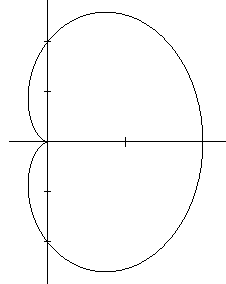
\includegraphics[width=6cm,keepaspectratio]{cardioid.png}
    \caption{カージオイド}
    \label{fig:cardioid}
  \end{center}
\end{minipage}
\begin{minipage}[b]{0.45\textwidth}
  \begin{center}
    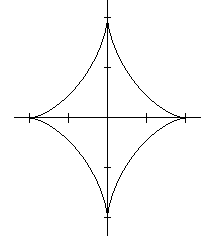
\includegraphics[width=6cm,keepaspectratio]{hypocycloid.png}
    \caption{4尖点の内サイクロイド}
    \label{fig:hypocycloid}
  \end{center}
\end{minipage}
\end{center}
\end{figure}
\begin{figure}
\begin{center}
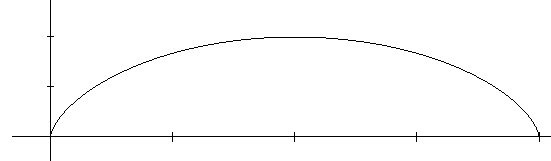
\includegraphics[height=4cm,keepaspectratio]{cycloid.png}
    \caption{サイクロイド}
    \label{fig:cycloid}
\end{center}
\end{figure}
\section{課題2}
\subsection{課題2-1}
テキストの展開図のように$A,B,C,D,H,I,J,G$を定める。$\triangle BCD$が正三角形であることから,$HB=IC=JD=\frac{\sqrt{3}}{2}w$である。三角形の重心は三角形の頂点と対辺の2等分点を結ぶ線分を$2:1$に内分するから,$GB=GC=GD=\frac{1}{\sqrt{3}}w$,$GH=GI=GJ=\frac{1}{2\sqrt{3}}w$となる。正四面体の高さAGは,三平方の定理より$AG=\sqrt{IA^2-IG^2}=\sqrt{\frac{2}{3}}w$となる。よって各頂点の位置は,
\begin{eqnarray*}
A:(\sqrt{\frac{2}{3}}w,0,0)\\
B:(0,\frac{1}{\sqrt{3}}w,0)\\
C:(0,-\frac{1}{2\sqrt{3}}w,\frac{w}{2})\\
D:(0,-\frac{1}{2\sqrt{3}}w,-\frac{w}{2})\\
\end{eqnarray*}
となる。

\subsection{課題2-2}
正四面体の重心は,
$$
\left( \frac{\sqrt{\frac{2}{3}}w+0+0+0}{4},\frac{0+\frac{1}{\sqrt{3}}w-\frac{1}{2\sqrt{3}}w-\frac{1}{2\sqrt{3}}w}{4},\frac{0+0+\frac{w}{2}-\frac{w}{2}}{4}\right)=\left(\frac{1}{4}\sqrt{\frac{2}{3}}w,0,0\right)
$$
重心が原点Oに一致するように各頂点を平行移動すると,
\begin{eqnarray*}
A':(\frac{1}{2}\sqrt{\frac{3}{2}}w,0,0)\\
B':(-\frac{1}{4}\sqrt{\frac{2}{3}}w,\frac{1}{\sqrt{3}}w,0)\\
C':(-\frac{1}{4}\sqrt{\frac{2}{3}}w,-\frac{1}{2\sqrt{3}}w,\frac{w}{2})\\
D':(-\frac{1}{4}\sqrt{\frac{2}{3}}w,-\frac{1}{2\sqrt{3}}w,-\frac{w}{2})\\
\end{eqnarray*}
ここで,半径1の球に内接する正四面体を考えているから,$A':(1,0,0)$である。よって,$w=2\sqrt{\frac{2}{3}}$となる。これを代入して,正四面体の頂点を求めると以下のようになる。
\begin{eqnarray*}
A':(1,0,0)\\
B':(-\frac{1}{3},\frac{2\sqrt{2}}{3},0)\\
C':(-\frac{1}{3},-\frac{\sqrt{2}}{3},\frac{\sqrt{6}}{3})\\
D':(-\frac{1}{3},-\frac{\sqrt{2}}{3},-\frac{\sqrt{6}}{3})
\end{eqnarray*}

\subsection{課題2-3}
ロボットアームの各パーツの登録部分をリスト\ref{armtouroku}に示す。

\begin{lstlisting}[caption=ロボットアームの各パーツの登録部分,label=armtouroku]
void init(void){
	myQuad=gluNewQuadric();
	gluQuadricDrawStyle(myQuad,GLU_LINE);
	glClearColor(1.0,1.0,1.0,1.0);
	gluLookAt(1,1,1,0,0,0,0,1,0);
	
	glNewList(ID_B,GL_COMPILE);
	glColor3f(0.0,0.0,0.0);
	glPushMatrix();
	glTranslatef(0.0, HEIGHT_B, 0.0);
	glScalef(0.5,HEIGHT_B,0.5);
	glRotated(90.0,1.0,0.0,0.0);
	gluCylinder(myQuad,1,1,2,50,4);
	glPopMatrix();
	glEndList();
	
	glNewList(ID_L,GL_COMPILE);
	glColor3f(0.0,0.0,0.0);
	glPushMatrix();
	glTranslatef(0.0,0.5*HEIGHT_L,WIDTH_L);
	glScalef(WIDTH_L,HEIGHT_L,WIDTH_L);
	glutWireCube(1.0);
	glPopMatrix();
	glEndList();
	
	glNewList(ID_U,GL_COMPILE);
	glColor3f(0.0,0.0,0.0);
	glPushMatrix();
	glTranslatef(0.0,0.5*HEIGHT_U,WIDTH_U);
	glScalef(WIDTH_U,HEIGHT_U,WIDTH_U);
	glutWireCube(1.0);
	glPopMatrix();
	glEndList();
}
\end{lstlisting}

次に,キーボードコールバック関数をリスト\ref{armkeycall}に示す。\texttt{SPEED}は定数マクロである。
\begin{lstlisting}[caption=キーボードコールバック関数,label=armkeycall]
void keyin(unsigned char key,int x,int y){
	switch(key){
		case '\033':
		case 'q':
		case 'Q':
		exit(0);
		break;
		case 'a':
		rotAng[0]+=SPEED;
		break;
		case 's':
		rotAng[0]-=SPEED;
		break;
		case 'd':
		rotAng[1]+=SPEED;
		break;
		case 'f':
		rotAng[1]-=SPEED;
		break;
		case 'h':
		rotAng[2]+=SPEED;
		break;
		case 'j':
		rotAng[2]-=SPEED;
		break;
	}
}
\end{lstlisting}
このキーボードコールバック関数を通じて各パーツの角度を変更し,テキストのリスト20のディスプレイ関数によって描画処理を行う。

描画されたロボットアームを図\ref{fig:armrobot}に示す。

\begin{figure}
\begin{center}
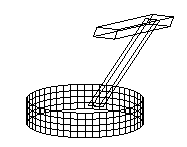
\includegraphics[height=5cm,keepaspectratio]{armrobot.png}
    \caption{描画されたロボットアーム}
    \label{fig:armrobot}
\end{center}
\end{figure}

\subsection{課題2-4}
実装したタイマコールバック関数をリスト\ref{timercallbuck}に示す。
\begin{lstlisting}[caption=タイマコールバック関数,label=timercallbuck]
static void timer(int dummy){
	glutTimerFunc(100,timer,0);
	glMatrixMode(GL_MODELVIEW);
	if (isAnime==1){
		rotAng[0]+=2.0;
		rotAng[1]=sin(speed)*10.0;
		rotAng[2]=sin(speed*4)*10.0;
		speed+=0.2;
	}
	glutPostRedisplay();
}
\end{lstlisting}
上腕を下腕より速く揺らすことによって,手を振って踊っているように見えると考えた。揺らす処理にはsin関数を用いた。また,台座も一定速度で回転させてみた。前節のキーボードコールバック関数の代わりに,タイマコールバック関数を呼び出すことで,踊っているような処理を実現した。


\section{課題3}
\subsection{課題3-1}
2つのベクトルの外積は,そのベクトルがなす平面の法線ベクトルになる。すなわち,3点$P_1,P_2,P_3$を含む平面の法線ベクトルは,$\overrightarrow{P_1 P_2}\times\overrightarrow{P_1 P_3}$によって求められる。よって,求めるすべての単位法線ベクトルは,
$$
\pm\frac{\overrightarrow{P_1 P_2}\times\overrightarrow{P_1 P_3}}{|\overrightarrow{P_1 P_2}\times\overrightarrow{P_1 P_3}|}
$$
となる。
\subsection{課題3-2}
右手系の外積で,$\overrightarrow{P_1 P_2}\times\overrightarrow{P_1 P_3}$が正となるとき表で,負となるとき裏であると判定できる。
\subsection{課題3-3}
ウェブサイト\cite{4}によれば,Phongの照光モデルはPhongの反射モデルとも呼ばれる,3次元コンピュータグラフィックスにおいて,モデリングされた面上の点に影をつけるための照明と陰影(シェーディング)モデルである。ユタ大学の理学博士であるBui Tuong Phongによって開発され,1973年に"Illumination for Computer Generated Pictures"の題で学位論文として発表された。

現実世界では,物体は光源からの光のほか,反射光などにより様々な方向から光が当たる。しかし,これらすべてをそのままプログラミングすることは難しいため,Phongの照光モデルによって単純化を行う。このモデルでは,面上の点における陰影を決定する際に,次のような単純化ができる利点がある。
\begin{itemize}
\item このモデルは,「局所的な」反射モデルである。すなわち,ラジオシティのようなレイトレーシングで行うような二次反射を計算する必要はない。反射した光の減衰を補正するために,外部の「環境光」(ambient) の項をレンダリングする際に加えている。
\item 表面からの反射を3つの項目,すなわち「鏡面反射」(specular reflection),「拡散反射」(diffuse reflection) と「環境反射」(ambient reflection) に分けている。
\end{itemize}
Phongの反射モデルの式は以下のようになる。
$$
I_p=k_a i_a + \sum_{\mathrm{lights}} (k_d (\bm{L}\cdot \bm{N})i_d + k_s(\bm{R}\cdot \bm{V})^\alpha i_s)
$$
各文字の定義を以下に示す。
\begin{eqnarray*}
I_p&:&表面上の各点における光の強度\\
k_s&:&鏡面反射係数。入射光に対する鏡面反射率\\
k_d&:&拡散反射係数。入射光に対する拡散反射率\\
k_a&:&環境反射係数。シーン全体を照らす環境光の反射率\\
i_a&:&環境光の照度\\
i_d&:&入射光の拡散反射成分\\
i_s&:&入射光の鏡面反射成分\\
\alpha&:&材質の光沢度。光沢のある点から反射する光がどのくらい均等に反射するか\\
\bm{L}&:&物体表面上の点からそれぞれの光源 (\mathrm{light}) への方向ベクトル\\
\bm{N}&:&表面上の点における法線\\
\bm{R}&:&面上のその点において光線が完全に反射 (\mathrm{reflect}) される方向\\
\bm{V}&:&視点に向かう方向
\end{eqnarray*}
総和記号は光源についてすべての和をとることを意味する。総和記号の外にある項が環境光の反射による強度についての項,総和記号の中の1項目が光源からの光の拡散反射に関する項,2項目が鏡面反射に関する項である。


\subsection{課題3-4}
頂点の法線ベクトルは,重心からその頂点に向かう向きとなる。よって,原点を中心とする半径1の円に内接する正多面体の頂点の法線ベクトルは,その頂点の位置ベクトルと一致する。正四面体,正六面体,正八面体を描画するプログラムの主要部をリスト\ref{seisimentai},\ref{seirokumentai},\ref{seihatimentai}にそれぞれ示す。

\begin{lstlisting}[caption=正四面体を描画するプログラム(主要部),label=seisimentai]
GLdouble vP[4][3]={{1.000,0.000,0.000},{-0.333,0.943,0.000}
,{-0.333,-0.471,0.816},{-0.333,-0.471,-0.816}};
int tP[4][3]={{0,1,2},{0,3,1},{0,2,3},{1,3,2}};

void display(void){
	int i,j;
	glClear(GL_COLOR_BUFFER_BIT|GL_DEPTH_BUFFER_BIT);
	glMatrixMode(GL_MODELVIEW);

	glBegin(GL_TRIANGLES);
	for(i=0;i<4;i++){
		for(j=0;j<3;j++){
			glNormal3dv(vP[tP[i][j]]);
			glVertex3dv(vP[tP[i][j]]);
		}
	}
	glEnd();
	glutPostRedisplay();
	glutSwapBuffers();

}
\end{lstlisting}
\begin{lstlisting}[caption=正六面体を描画するプログラム(主要部),label=seirokumentai]
GLdouble vP[8][3]={{-0.577,-0.577,0.577},{0.577,-0.577,0.577}
,{0.577,-0.577,-0.577},{-0.577,-0.577,-0.577},{-0.577,0.577,0.577}
,{0.577,0.577,0.577},{0.577,0.577,-0.577},{-0.577,0.577,-0.577}};
int tP[6][4]={{3,2,1,0},{0,1,5,4},{1,2,6,5},{4,5,6,7},{3,7,6,2},{0,4,7,3}};


void display(void){
	int i,j;
	glClear(GL_COLOR_BUFFER_BIT|GL_DEPTH_BUFFER_BIT);
	glMatrixMode(GL_MODELVIEW);

	glBegin(GL_QUADS);
	for(i=0;i<6;i++){
		for(j=0;j<4;j++){
			glNormal3dv(vP[tP[i][j]]);
			glVertex3dv(vP[tP[i][j]]);
		}
	}
	glEnd();
	glutPostRedisplay();
	glutSwapBuffers();

}
\end{lstlisting}
\begin{lstlisting}[caption=正八面体を描画するプログラム(主要部),label=seihatimentai]
GLdouble vP[6][3]={{1,0,0},{0,1,0},{0,0,1},{-1,0,0},{0,-1,0},{0,0,-1}};
int tP[8][3]={{0,1,2},{5,1,0},{3,1,5},{2,1,3},{2,4,0},{0,4,5},{5,4,3},{3,4,2}};


void display(void){
	int i,j;
	glClear(GL_COLOR_BUFFER_BIT|GL_DEPTH_BUFFER_BIT);
	glMatrixMode(GL_MODELVIEW);

	glBegin(GL_TRIANGLES);
	for(i=0;i<8;i++){
		for(j=0;j<3;j++){
			glNormal3dv(vP[tP[i][j]]);
			glVertex3dv(vP[tP[i][j]]);
		}
	}
	glEnd();
	glutPostRedisplay();
	glutSwapBuffers();

}
\end{lstlisting}
\texttt{vP}に頂点の位置,\texttt{tP}にトポロジ情報を格納している。正六面体,正八面体の頂点の位置,トポロジ情報は,演習19で求めたものである。法線ベクトルの指定には,\texttt{vP}をそのまま利用している。描画された正四面体,正六面体,正八面体をそれぞれ図\ref{fig:seisimentai},\ref{fig:seirokumentai},\ref{fig:seihatimentai}に示す。

\begin{figure}[htbp]
\begin{center}
\begin{minipage}[b]{0.45\textwidth}
  \begin{center}
    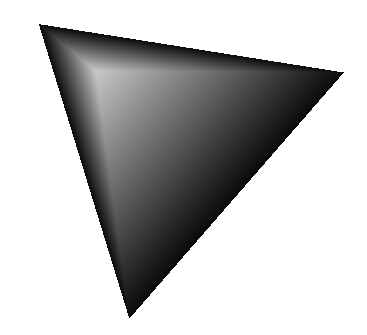
\includegraphics[width=4cm,keepaspectratio]{seisimentai.png}
    \caption{正四面体}
    \label{fig:seisimentai}
  \end{center}
\end{minipage}
\begin{minipage}[b]{0.45\textwidth}
  \begin{center}
    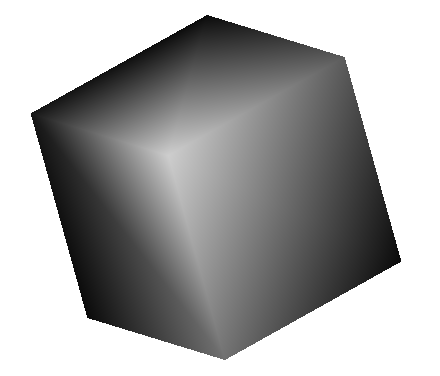
\includegraphics[width=4cm,keepaspectratio]{seirokumentai.png}
    \caption{正六面体}
    \label{fig:seirokumentai}
  \end{center}
\end{minipage}
\begin{minipage}[b]{0.45\textwidth}
  \begin{center}
    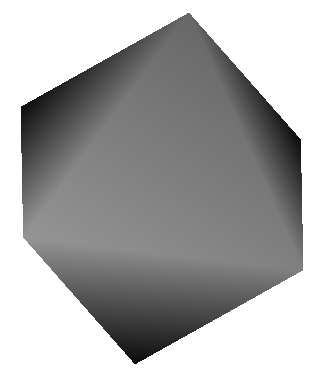
\includegraphics[width=4cm,keepaspectratio]{seihatimentai.png}
    \caption{正八面体}
    \label{fig:seihatimentai}
  \end{center}
\end{minipage}
\end{center}
\end{figure}

\subsection{課題3-5}
各パーツを回転させることができるように各パーツの回転角度を格納する変数\texttt{rotAng}をグローバル変数として定義し,display関数内での各パーツの呼び出し前に\texttt{glRotated}関数を挿入した。他の部分はテキストのリスト27と同じである。テキストのリスト27との変更部分をリスト\ref{real}に示す。
\begin{lstlisting}[caption=リアルなロボットアームを描画するプログラム(変更部分),label=real]
GLdouble rotAng[3]={0};

void display(void){
	glClear(GL_COLOR_BUFFER_BIT|GL_DEPTH_BUFFER_BIT);
	glMatrixMode(GL_MODELVIEW);
	glLoadIdentity();
	gluLookAt(1.0,1.0,1.0,0.0,0.5,0.0,0.0,1.0,0.0);
	glRotated(rotAng[0],0,1,0);
	glCallList(ID_B);
	glTranslatef(0.0,HEIGHT_B,0.0);
	glRotated(rotAng[1],0,0,1);
	glCallList(ID_L);
	glTranslatef(0.0,HEIGHT_L,0.0);
	glRotated(rotAng[2],0,0,1);
	glCallList(ID_U);
	glutSwapBuffers();
}
\end{lstlisting}

描画されたロボットアームを図\ref{fig:3Drobotarm}に示す。
\begin{figure}
\begin{center}
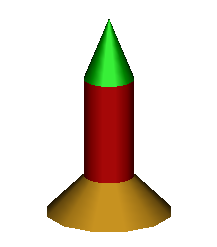
\includegraphics[height=5cm,keepaspectratio]{real.png}
    \caption{リアルなロボットアーム(ロケット?)}
    \label{fig:3Drobotarm}
\end{center}
\end{figure}
\section{感想}
これまで履修してきた情報系の授業に比べて,グラフィックスに関する内容が多かったため,実装したことが視覚的に強く反映されたので,楽しかった。一応C言語ではあるものの,初めて扱うOpenGLの関数が多く出てきて難しかった。
今後もプログラミングをする場面がたくさんあると思うので,継続的にプログラミング技術を高めていきたいと思った。

\section{改善案}
付録として,主要なOpenGLの関数がまとめてあると便利だと思いました。あと,授業内容とは少しずれますが,4年生も履修可能な科目にしてもいいと思いました。
\begin{thebibliography}{99}
\bibitem{1} https://qiita.com/keitean/items/2f95dfb2944895f001e7
\bibitem{2} https://eng-entrance.com/linux-command-grep
\bibitem{3} https://kazmax.zpp.jp/cmd/t/touch.1.html
\bibitem{4} https://ja.wikipedia.org/wiki/Phong\%E3\%81\%AE\%E5\%8F\%8D\%E5\%B0\%84\%E3\%83

\%A2\%E3\%83\%87\%E3\%83\%AB
\bibitem{6} 高橋章,R03-Ec5 プログラミング演習$\rm I\hspace{-.01em}I$テキスト
\end{thebibliography}

\end{document}


\begin{lstlisting}[caption=,label=]

\end{lstlisting}

